\documentclass[sigconf,nonacm]{acmart}

\AtBeginDocument{%
\providecommand\BibTeX{{%
\normalfont B\kern-0.5em{\scshape i\kern-0.25em b}\kern-0.8em\TeX}}}



\newcommand{\scores}{\textsc{SCORES}}

\usepackage{verbatim}
\usepackage[linesnumbered, boxed, resetcount]{algorithm2e}
\usepackage{hyperref}

\usepackage{listings}
\usepackage{xcolor}

\usepackage{amsmath}
\usepackage{graphicx}

%* Package settings
\hypersetup{
colorlinks  = true,
linkcolor   = black,
urlcolor    = red,
}

\begin{document}

\title{Activity Bot's Catch Game}

\author{Bruno Silva \\ \href{https://github.com/brunofavs/propeller_cath_game}{Github Repository} }
\email{bruno.silva1@student.um.si}
\affiliation{%
    \institution{Faculty of Electrical \\Engineering and Computer Science,\\
    University of Maribor\\Koro\v{s}ka cesta 46}
    \city{SI-2000 Maribor}
    \country{Slovenia}
    }

    
    
    \begin{abstract}
    
This paper describes the development of two small robots from \textit{Parallax}, the \textit{Activity
Bots} - a seeker and a runner
- that use ultrasonic sensors to play the \textit{Catch game}. The seeker robot was
programmed to detect the runner robot and chase it, while the runner robot was
programmed to evade the seeker robot. The paper discusses the design and
construction of the robots and the algorithms used to control their movements.
The results of experiments conducted to test the robots' performance in the game
are presented and analyzed. The experiments show that the seeker robot was able
to detect and pursue the runner robot successfully.
This paper also goes briefly on how to incorporate the workflow of parallax's
robots programming in the engineer's favorite VScode.
 

    \end{abstract}
    
    \maketitle


    \keywords{\LaTeX, template, paper, conference }

\section{Introduction}

    Targeting and following algorithms are the base for many
    applications in robotics field. While RGBD cameras or 2D/3D LiDARs are often
    the preferred choice for most applications, ultrasonic sensors, even though
    simple and quite less powerful, are sometimes a good alternative due to
    their much more affordable price. The approach used in this research has
    some reassemblance with the working principles of stereo cameras. Using 1
    ultrasonic sensor proved insufficient to predict the target's direction.
    Switching to 2 sensors and measuring deltas instead of absolute values
    allowed the seeker to perceive the direction the target was coming from.
    This working principle will be further expanded on in the seeker's robot
    chapter of this paper.

\begin{figure}[h]
    \centering
    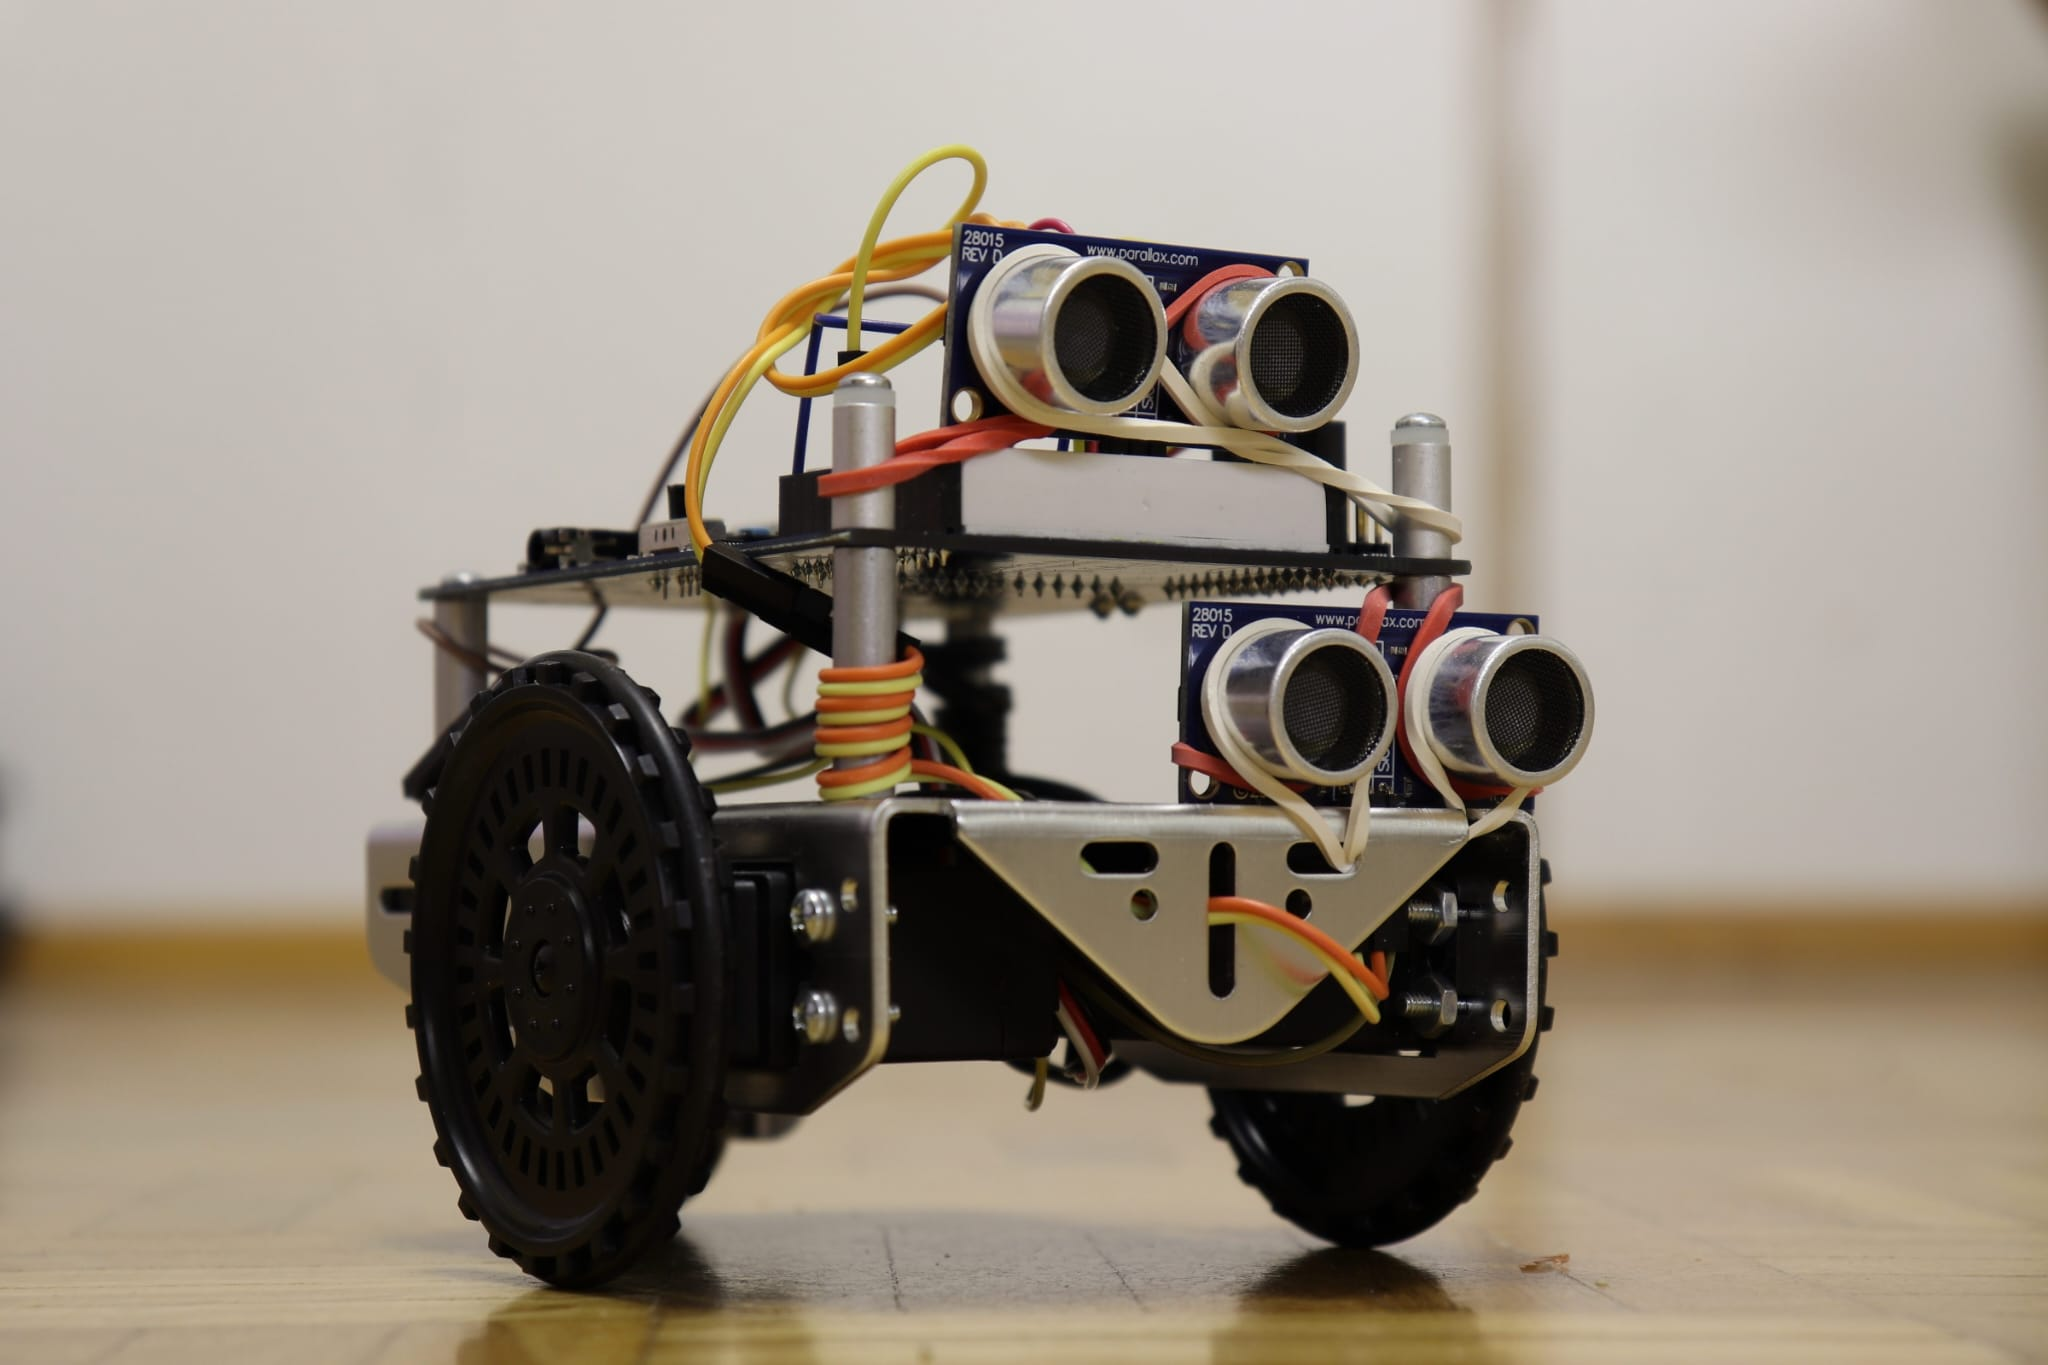
\includegraphics[scale=0.1]{resources/Seeker_robot/4.jpeg}
    \caption{\label{fig:Seeker}Seeker Robot.}
\end{figure}

\begin{figure}[h]
    \centering
    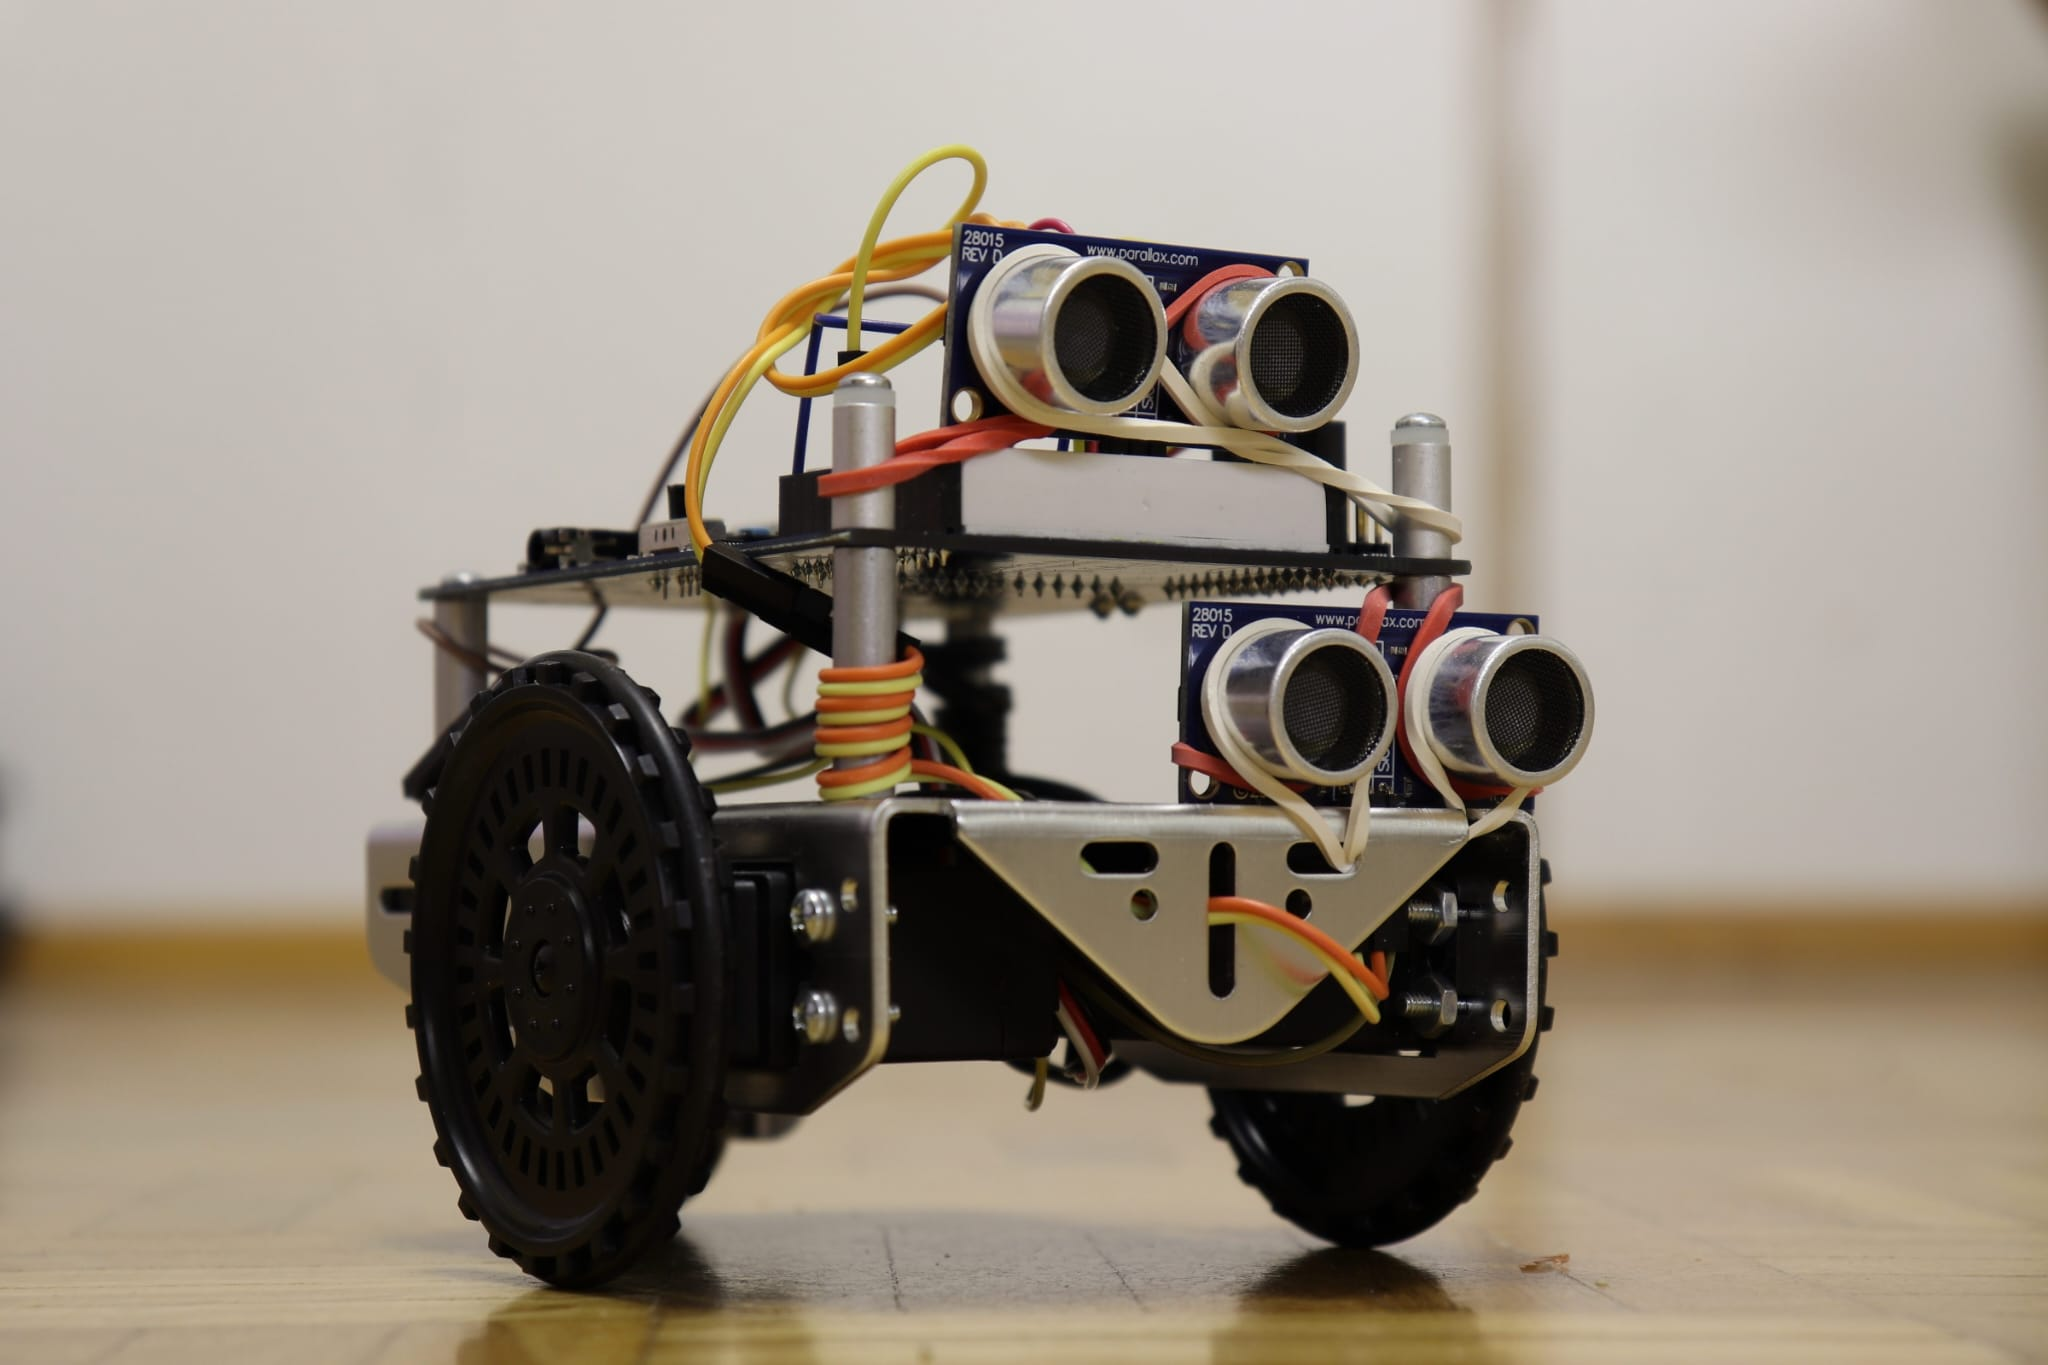
\includegraphics[scale=0.1]{resources/Seeker_robot/4.jpeg}
    \caption{\label{fig:Runner}Runner Robot. PLACEHOLDER IMG}
\end{figure}

\section{Developing Environment}

      This chapter is meant to explain the working environment of the
      programming
      of Parallax's robots and the work flow that was used throughout this
      project
      

      \subsection{SimpleIDE}

      SimpleIDE is Parallax's official developing platform. As the name
      suggests, it's a rather simple and feature lacking IDE, meant for absolute
      beginners. Basic features like autocompletion, keyword highlight, or even
      error squiggles are not present. This combined with the lack of
      customization makes a more experienced user rather frustrated when trying
      to develop on this platform. 

      \begin{figure}[h]
            \centering
            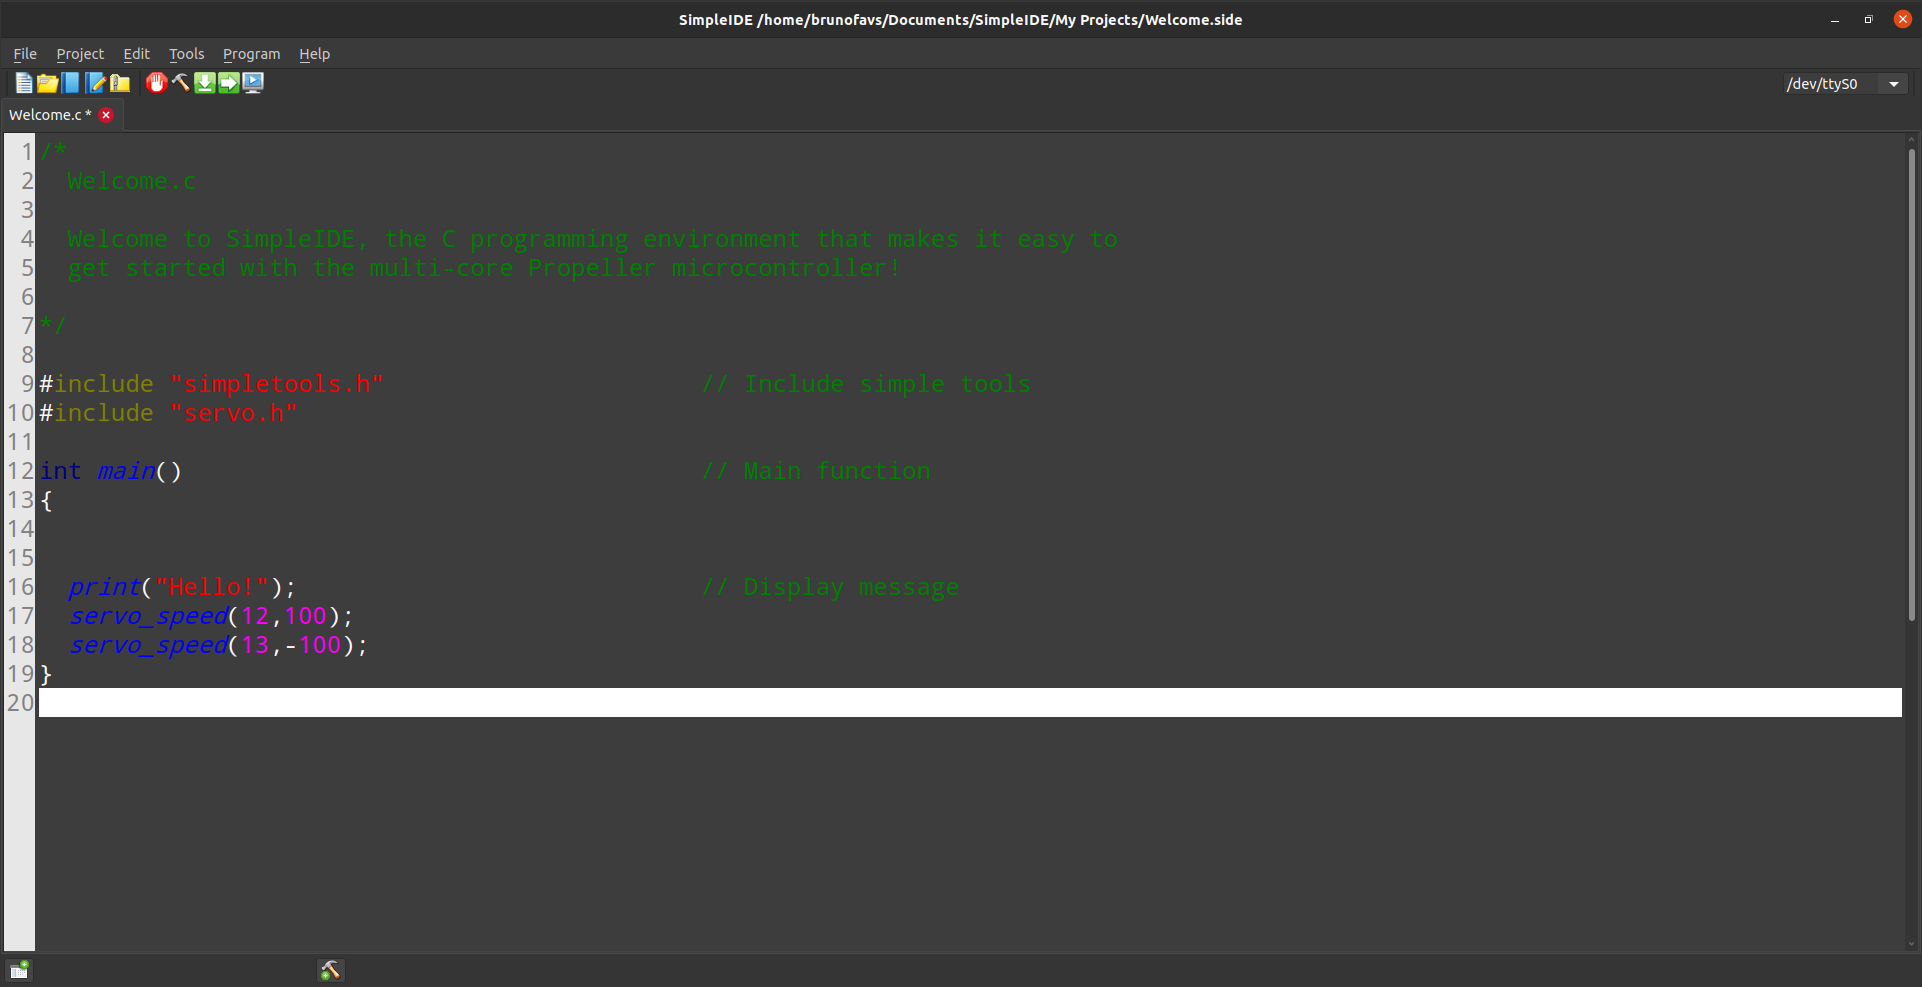
\includegraphics[scale=0.1]{resources/simple_ide.png}
            \caption{\label{fig:simple_ide}SimpleIDE working environment.}
      \end{figure}


      \subsection{VScode Integration}

      Fortunately, it is possible, with some workarounds, to migrate the grand
      majority of the workflow into a more advanced environment like VScode.
      
      \begin{enumerate}
            \item PlatformIO
                  \begin{itemize}
                        \item PlatformIO's IDE is a VScode
                        extension which transforms VScode into a IDE capable of
                        fully programming a wide range of microcontrollers, from
                        code writting to EEPROM flashing. There's a platform
                        there for working the Parallax's
                        microcontrollers (\href{https://github.com/msquirogac/platform-propeller}{Github}).
                        However, upon exhaustive testing this platform seems to
                        be a half finished attempt which doesn't work.
                  \end{itemize}
            \item VScode
                  \begin{itemize}
                        \item One way is to add SimpleIDE's libraries to the
                        default C path for the default C libraries. This
                        approach is better for long term development, but on
                        this project wasn't used.

                        \item Another way is to import the libraries straight
                        into the project's folder, allowing VScode to treat them
                        as user built libraries.
                        
                        This was the approach used. To replicate the following
                        folders have to be copied to the project folder:
                        \begin{itemize}
                              \item \begin{lstlisting}[language=bash]
$ /home/${USER}/Documents/SimpleIDE/Learn
$ /opt/parallax
                                    \end{lstlisting}
                              \end{itemize}
                              It's important to note that this applies only for Ubuntu
                                    based systems and that both these folders should be
                                    added to the repository's \textit{.gitignore} as they
                                    are quite big and not important to the project itself.
                  \end{itemize}
      \end{enumerate}


\section{Seeker Robot}


\subsection{Algorithm Explanation}

The core of the seeker's algorithm is based on 2 functions:
\begin{enumerate}
      \item Assessing targets in range of ultrasonic sensors;
      
      This involves stopping, getting 2 measurements from each sensor spaced by
      a predefined $\Delta t\space[s]$, calculating the $\Delta d\space[cm]$ from the right and
      left sensor and figure out which direction the target is coming from and
      outputting accordingly.
      \item Giving moving order to the servos to chase the target. This function
      purpose is to, given the direction the target crossed from, tune how much
      the robot should rotate and go forward. This ideally would be dynamically
      controlled, but since the robot cannot know how fast the target crossed,
      it has to be manually tuned for a given target velocity.
\end{enumerate}

\subsection{Function targetAssessing()}

The first thing this function does is assure the robot is still before reading
the differential distance measures. The code could account for the velocity of
the seeker and correct the measure, but that would be mathematically a lot more
challenging.

Then, after reading the distance measurements, the robot could be left with 5
possible case-scenarios given the 2 differential measures :

\begin{enumerate}
     \item $\Delta D_L<0 \wedge \Delta D_R \approx 0$ \\ This would mean the
     target came from out of range and is started being detected the by left
     sensor, since the measure distance reduced. The robot should thus
     turn \textbf{RIGHT};
     
     \item $\Delta D_L\approx 0\wedge \Delta D_R < 0$ \\ This would mean the same
     as case 1, but instead the target is approaching from the right, so the
     robot should turn \textbf{LEFT};

     \item $\Delta D_L>0\wedge \Delta D_R \approx 0$ \\ This would mean the
     target was already in sight of the left sensor and left suddenly to the
     left, allowing the sensor to see into the further away background. This
     would mean the robot should turn \textbf{LEFT};
     
     \item $\Delta D_L\approx 0 \wedge \Delta D_R > 0$ \\ This would mean the
     target was already in sight of the right sensor and left suddenly to the
     right, allowing the sensor to see into the further away background. This
     would mean the robot should turn \textbf{RIGHT};

     \item $|\Delta D_L|>0\wedge |\Delta D_R| > 0$ \\ This would mean that the
     target is currently in front of the robot and is either getting further
     away or getting closer. Either way, for the seeker robot the order should
     be to go \textbf{forward}.
\end{enumerate}

In practice, a \textit{threshold} was used instead of 0, to account for sensor
measurement error.


\subsection{Measuring distances}

Initially, in order to assure the robot could always read the latest reading from the
sensor when needing to evaluate distances, and to take advantage of the
parallax's multicore chip, the sensor data was being stored on a global variable
that was constantly being updates parallel to the code. The code for acquiring
data was running on a separate core. 
However, due to timing reasons, this proved to be more harmful to the overall
performance of the robot. In the end, whenever the robot isn't actively pursuing
the target, he is in a semi-idle state doing nothing other than to measure
distances to try to identify a potential target.

\subsection{Issues with the current implementation}
\begin{itemize}
      \item 
      As of right now, the seeker isn't identifying how close the target is. As of
      right now, the robot upon identifying the target's direction, its servos get an
      input for a set amount of time at a set power. A runner coming into frame
      further away should result in a smaller turn time while another closer away
      should result in a sharper turn.
      Finding a function that correlates the distance to the correct turn amount
      is not an easy task tho, a trial and error approach could be used, but
      such approach is reckoned to be too volatile and sensitive to environment changes.

      \item Using ultrasonic sensors instead of cameras basically limits the
      robot perception field into a line instead of spacial. This is means if for
      some reason the runner gets completely out of the runner field of view,
      the seeker becomes clueless again until the runner comes back into frame
      again.
      One approach to this problem could be to have the seeker pan around itself
      whenever he got more than a set amount of repeated null differential
      distances readings.

      \item The ultrasonic sensors used are not very accurate and from time to
      time yield outrageous readings, the robot if left facing a plain wall
      still for a big enough period of time, its almost certain that he will
      spontaneously turn because of an inaccurate reading. The sensors were
      replaced and switched and the problem remained.
\end{itemize}



\section{Runner Robot}

This robot does not possess any intelligence, it's just working as dummy robot
that goes around in circles to provide the seeker something to follow. The only
possible mounting position that would somewhat suit this robot is facing
backwards, as there is never a scenario where the runner wants to be facing the
seeker, but even then the runner ideally shouldn't be directly in front of the 
seeker, since it would be in its perception field. 

\section{Experiments}

The following section goes over how the algorithm performed when faced with a
few tests. It was tested the reaction time and the accuracy of the assessing,
meaning if the seeker determined the right runner's direction.\footnote[1]{There
are demo videos in the Github Repository}


\subsection{Reaction time}

It's important to note the following : the reaction time is mainly controlled by
the delay between differential measures, \textit{$ \Delta T$}. In theory with a really low $ \Delta T$, the
response time would be really great. In practice, this proved to have a lot more
drawbacks:
\begin{itemize}
      \item The runner robot is not 100\% opaque, meaning its hollowness makes
      the robot's behavior with a low  $ \Delta T$ unpredictable.

      \item A low $ \Delta T$ also makes the robot's behavior very jittery and nervous.
      
\end{itemize}

Nevertheless, with a delay of \textit{50ms}, here are some measurements of the
response time with a slow moving object.


\Large{
INSERT RESULTS HERE}



 
\subsection{Accuracy of target assessing}

To test the seeker's accuracy, a series of objects approached the seeker from
different angles and speeds and here are some results:


\Large{
INSERT RESULTS HERE}


\section{Conclusions}


% \bibliographystyle{ACM-Reference-Format}
% \bibliography{references}

\end{document}
